%%%% CS553 Cryptography Term Paper TEMPLATE %%%%

%%%% 1. DOCUMENTCLASS %%%%
\documentclass[preprint]{transcrypto}
\documentclass{homeworg}
\documentclass{article}
\usepackage{graphicx}
\graphicspath{ {./images/} }
\graphicspath{ {../assets/} }
%%%% NOTES:
% - Change "submission" to "final" for final version
% - Add "spthm" for LNCS-like theorems


%%%% 2. PACKAGES %%%%
% \usepackage{lipsum} % Example package -- can be removed
\usepackage{hyperref}

%%%% 3. AUTHOR, INSTITUTE %%%%
\author{Ambar Mutha \and Ashutosh Sahu \and Priyanka Yadav}
\institute{
  IIT Bhilai, Raipur, India, \email[ambarm@iitbhilai.ac.in,ashutoshsahu@iitbhilai.ac.in,priyankay@iitbhilai.ac.in]{{ambarm,ashutoshsahu,priyankay}@iitbhilai.ac.in}
}
%%%% NOTES:
% - We need a city name for indexation purpose, even if it is redundant
%   (eg: University of Atlantis, Atlantis, Atlantis)
% - \inst{} can be omitted if there is a single institute,
%   or exactly one institute per author


%%%% 4. TITLE %%%%
\title{Analysis of SQUARE}
%%%% NOTES:
% - If the title is too long, or includes special macro, please
%   provide a "running title" as optional argument: \title[Short]{Long}
% - You can provide an optional subtitle with \subtitle.

\begin{document}

\maketitle


%%%% 5. KEYWORDS %%%%
\keywords{SQUARE \and Block cipher \and SPN}


%%%% 6. ABSTRACT %%%%
\begin{abstract}
  In this paper we analyse the cipher SQUARE and various attacks on it.

  % \lipsum[8]
\end{abstract}


%%%% 7. PAPER CONTENT %%%%
%%%\section{Introduction}
\begin{document}

\maketitle
\paragraph{ Introduction of Square Cipher:-\\}
\\
Square is an iterated block cipher. Block length is 128 bits and key length also 128 bits. The round transformation of Square is composed of four distinct transformations($\theta$,$\gamma$,$\pi$,$\sigma$). We wil combine these four building blocks in a single set of table-lookups and exor operations. The basic building blocks of the cipher are five different invertible transformations that operate on a 4x4 array of bytes. 
\paragraph{ Transformation Operations:-}\\
\paragraph{1.1 A Linear Transformation ($\theta$) :- \\} \\
$\theta$ is a linear operation. We have state matrix $a$ and $\theta$ operates on each of four rows separately. Expression for $\theta$ operation:- 
$$
\theta: b=\theta(a) \Leftrightarrow b_{i, j}=c_{j} a_{i, 0} \oplus c_{j-1} a_{i, 1} \oplus c_{j-2} a_{i, 2} \oplus c_{j-3} a_{i, 3}
$$
The element of a state a in row $i$ and column $j$ is specified as $a_{i, j}$ . Both indexes start from $0$.\\
where, the multiplication is in GF $\left(2^{8}\right)$, which is also called the Galois field and the coefficients of $c$ must be taken modulo $4 .$ Here, addition in the field is exclusive XOR.\\
$c$ is a 1D array and equivalent to below matrix:-  \\
                                %  $c$   $\equiv$\\
                               
                                $c$   $\equiv$ \begin{bmatrix}
                                                2 & 1 & 1 & 3\\
                                                3 & 2 & 1 & 1\\
                                                1 & 3 & 2 & 1\\
                                                1 & 1 & 3 & 2\\
                                                \end{bmatrix}
                                                
We can denote every row of a state as a polynomial.like, the polynomial corresponding to row $i$ of a state $a$ is given by
$$
a_{i}(x)=a_{i, 0} \oplus a_{i, 1} x \oplus a_{i, 2} x^{2} a_{i, 3} x^{3}
$$
Using this notation, and defining $c(x)=\oplus_{j} c_{j} x^{j}$ we can describe $\theta$ as a modular polynomial multiplication:
$$
b=\theta(a) \Leftrightarrow b_{i}(x)=c(x) a_{i}(x) \bmod 1 \oplus x^{4} \quad \text { for } \quad 0 \leq i<4
$$
The inverse of $\theta$ corresponds to a polynomial $d(x)$ given by
$$
d(x) c(x)=1 \quad\left(\bmod 1 \oplus x^{4}\right)
$$
\paragraph{1.2 A Nonlinear Transformation ($\gamma$):- \\}\\
$\gamma$ is a nonlinear byte substitution, identical for all bytes. We have
$$
\gamma: b=\gamma(a) \Leftrightarrow b_{i, j}=\mathrm{S}_{\gamma}\left(a_{i, j}\right)
$$
Here, $\mathrm{S}$ -box is an invertible 8-bit substitution table. 
The inverse of $\gamma$ consists of the application of the inverse substitution $\mathrm{S}_{\gamma}^{-1}$ to all bytes of a state.

\paragraph{1.3 A Byte Permutation ($\pi$):-\\}\\
$\pi$ is a linear operation. It transposes a matrix.
The effect of $\pi$ is the interchanging of rows and columns of a state. 
$$
\pi: b=\pi(a) \Leftrightarrow b_{i, j}=a_{j, i}
$$
$\pi$ is an involution,because transpose of transpose of a matrix is matrix itself.\\
hence $\pi^{-1}=\pi$

\paragraph{1.4 Bitwise Round Key Addition ($\sigma$):- \\}\\
$\sigma$ is a linear opeartion.\\
$\sigma\left[k^{t}\right]$ consist of the bitwise addition or $\xor$ of a round key $k^{t} .$ We have
$$
\sigma\left[k^{t}\right]: b=\sigma\left[k^{t}\right](a) \Leftrightarrow b=a \oplus k^{t}
$$
$\sigma$ is an involution also hence,
the inverse of $\sigma\left[k^{t}\right]$ is $\sigma\left[k^{t}\right]$ itself.
\paragraph{The Round Key Evolution ($\psi$):- \\}\\
The round keys $k^{t}$ are derived from the cipher key $K$. $k^{0}$ equals the cipher key $K$. The other round keys are derived iteratively by means of the invertible affine transformation $\psi$.
$$
\psi: k^{t}=\psi\left(k^{t-1}\right)
$$
\paragraph{First round :- \\}\\
There are total eight rounds in SQUARE cipher proceeded by a key addition $\sigma\left[k^{0}\right]$ and by $\theta^{-1}$ .
All four building blocks are composed into the round transformation. Every round is denoted by $\rho\left[k^{t}\right]$. We are doing just four transformation($\theta$,$\gamma$,$\pi$,$\sigma$) in every round.
$$
\rho\left[k^{t}\right]=\sigma\left[k^{t}\right] \circ \pi \circ \gamma \circ \theta
$$
The $\theta^{-1}$ before $\sigma\left[k^{0}\right]$ in SQUARE can be incorporated in the first round. We have
$$
\begin{aligned}
\rho\left[k^{1}\right] \circ \sigma\left[k^{0}\right] \circ \theta^{-1}\\ &=\sigma\left[k^{1}\right] \circ \pi \circ \gamma \circ \theta \circ \sigma\left[k^{0}\right] \circ \theta^{-1} \\
&=\sigma\left[k^{1}\right] \circ \pi \circ \gamma \circ \sigma\left[\theta\left(k^{0}\right)\right]
\end{aligned}
$$
Hence the initial $\theta^{-1}$ can be discarded by omitting $\theta$ in the first round and applying $\theta\left(k^{0}\right)$ instead of $k^{0} .$ 
Here,$k^{0}$ equals to Cipher key $K$.

SQUARE Cipher after complete eight rounds:-\\
$$
\operatorname{SQUARE}[k]=\rho\left[k^{8}\right] \circ \rho\left[k^{7}\right] \circ \rho\left[k^{6}\right] \circ \rho\left[k^{5}\right] \circ \rho\left[k^{4}\right] \circ \rho\left[k^{3}\right] \circ \rho\left[k^{2}\right] \circ \rho\left[k^{1}\right] \circ \sigma\left[k^{0}\right] \circ \theta^{-1}
$$
\\
   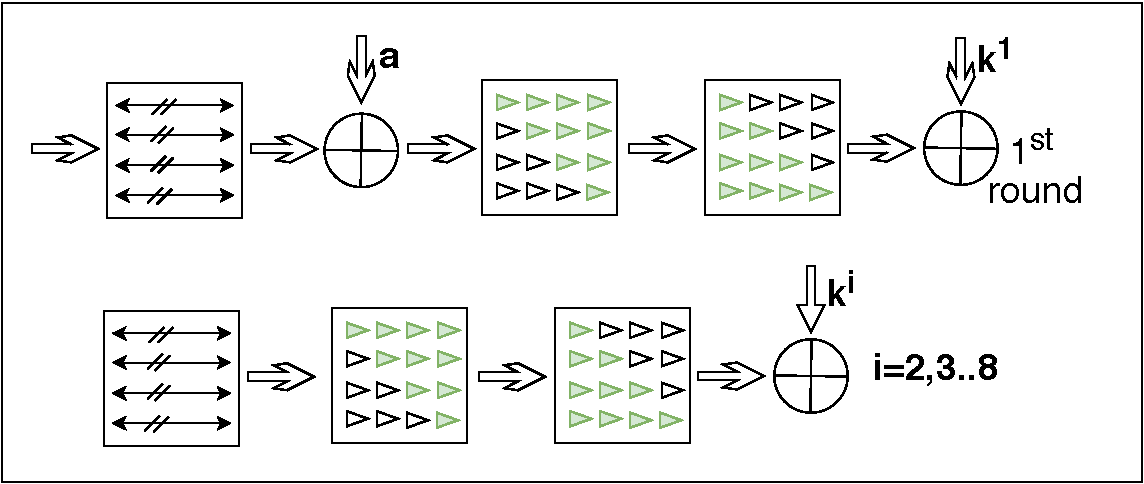
\includegraphics[width=0.9\columnwidth]{Square_cipher_diagram}\\
here, a is initial state matrix ,$k_{0}$ is cipher key, and $k_{1}$,$k_{2}$, .... , $k_{8}$ are round keys derived using key scheduling algorithm.\\
Only First round is different, but in others same transformation operations are applied in same order.

\end{document}




Widely used primitives like the AES~\cite{AES} do not have perfect
security, and can be analysed with linear
cryptanalysis~\cite{EC:Matsui93}, differential
cryptanalysis~\cite{JC:BihSha91}, or differential power
analysis~\cite{C:KocJafJun99}.  We show that the One-Time-Pad is
unconditionally secure in \autoref{sec:main}.

% \lipsum[9]

\section{Main Result}
\label{sec:main}

\section{Properties}
\subsection{DDT}
The Difference Distribution Table (DDT) has the highest value 4. Therefore, the maximum probabilty of a characteristic for difference across a single substitution $\frac{4}{256}$.

\begin{itemize}
  \item For each non-zero input difference, the maximum value of 4 occurs exactly once, 2 occurs 126 times and 0 occurs 129 times.
  \item For each non-zero output difference, the maximum value of 4 occurs exactly once, 2 occurs 126 times and 0 occurs 129 times..
  \item There are 33,150 zeroes in the DDT. Hence, roughly half of the input/output difference pairs are impossible.
\end{itemize}

The S-Box for SQUARE is different from that of AES but similar as these three properties are also followed the AES S-Box. The complete DDT can be seen at the \href{https://github.com/supercoww/square-term-paper/blob/master/code/scripts/ddt.txt}{Github repository}.

% \lipsum
\section{The Integral Attack}
This chosen plaintext attack attack was first introduced with the cipher SQUARE~\cite{FSE:DaeKnuRij97} and hence also known as the SQUARE attack. The basic attack is of 4 rounds which can be extended to 6 rounds.

A set $\Lambda$ of 256 plaintexts is chosen such that the first byte position in different plaintexts include all 256 values, and hence said to have the All property. All other positions have the constant property which means that all 256 values are same for that position.


\begin{figure}
  \centering
  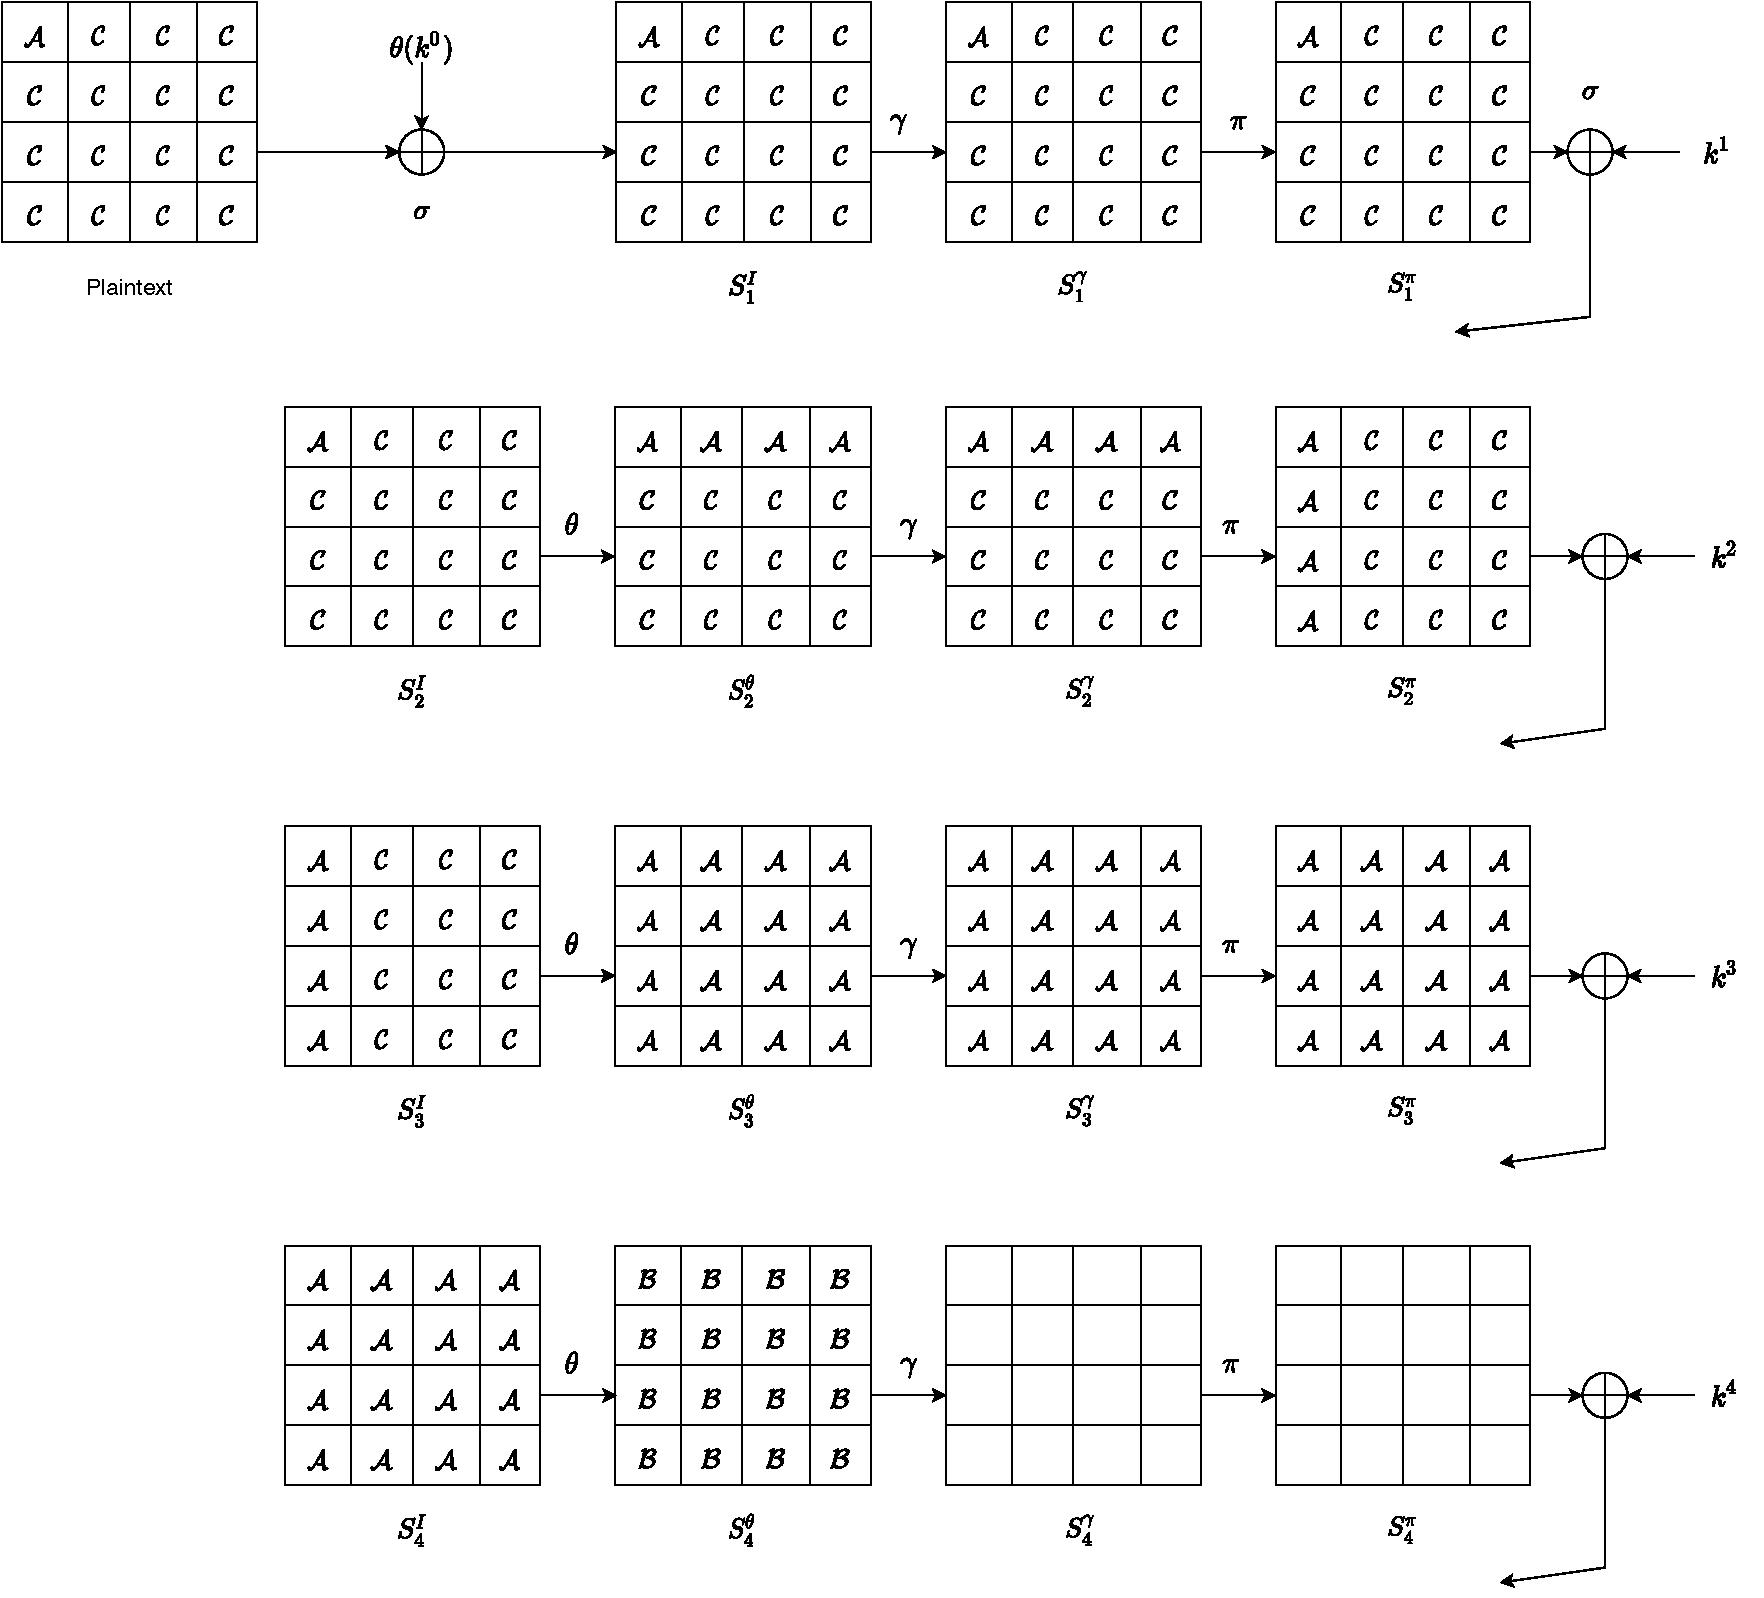
\includegraphics[width=\linewidth]{square_attack}
  \caption{Integral attack characteristic for 4 rounds}
  \label{fig:square_attack}
\end{figure}

\begin{flalign*}
  P_0 &= (0, c_1, c_2 \dotsc c_{15})\\
  P_1 &= (1, c_1, c_2 \dotsc c_{15})\\
  P_2 &= (2, c_1, c_2 \dotsc c_{15})\\
  &\vdots\\
  P_{255} &= (255, c_1, c_2 \dotsc c_{15})
\end{flalign*}

\begin{equation*}
  \Lambda = \{P_0, P_1, P_2 \dotsc P_{255}\}
\end{equation*}

The properties propagate through the rounds as shown in \autoref{fig:square_attack}. At the beginning of 4th round, all 16 positions have the All property. After the linear transformation $\theta$, all 16 positions have the balanced property as shown in \autoref{eq:bal}. A position is balanced if XOR sum of all 256 values is 0. It should be noted that All implies Balanced but the converse is not true.

\begin{flalign}
  \bigoplus_{0 \leq n \leq 255} S_{4,n}^\theta[i,j]
  &= \bigoplus_{0 \leq n \leq 255} \bigoplus_k c_{j-k} S_{4,n}^I[i,k] \label{eq:bal} \\
  &= \bigoplus_l c_l \bigoplus_{0 \leq n \leq 255} S_{4,n}^I[i,l+j] \nonumber \\
  &= \bigoplus_l c_l 0 \nonumber \\ &= 0 \nonumber
\end{flalign}

In the 4 round attack, we guess the value of a single byte $k_{i,j}^4$ of the round key $k^4$. Using $k_{i,j}^4$, we calculate the value of $S_4^\theta[j,i]$ for all 256 ciphertexts.

\begin{equation*}
  S_4^\theta[j,i] = Sbox^{-1}[S_5^I[i,j] \oplus k_{i,j}^4]
\end{equation*}

We verify whether the key guess was correct by calculating the XOR sum of all 256 values of $S_4^\theta[j,i]$. The key guess is discarded if the sum is non-zero. This is repeated for all bytes of the $k^4$. $k^4$ can be uniquely determined by using 2 $\Lambda$ sets of 256 plaintexts. Since the key schedule $\psi$ is invertible, the previous keys $k^0$ to $k^3$ can also be derived from $k^4$.

The attack can be extended from behind by guessing 4 bytes of $k^4$ and 4bytes of $k^5$ each time. 5 sets of 256 plaintexts are required for determining the key.

Another extension is possible from the beginning which involves crafting set of $2^32$ plaintexts such that the output of the first round has a column whose 4 byte value follows All property and the rest are Constant.

The complexity of different variations of the integral attack as in ~\cite{FSE:DaeKnuRij97} is shown in \autoref{tab:complexity}.

\begin{table}
  \centering
  \begin{tabular}{|c|c|c|c|}
    \hline
    Attack          & Plaintexts & Time  & Memory \\
    \hline
    4-round         & $2^9$      & $2^9$ & negl   \\
    5-round  type 1 & 211        & 240   & negl   \\
    5-round  type 2 & 232        & 240   & 232    \\
    6-round         & 232        & 272   & 232    \\
    \hline
  \end{tabular}

  \caption{Complexity of integral attack on SQUARE}
  \label{tab:complexity}
\end{table}

\section{Other Attacks}
\subsection{Related Key Boomerang Attack}
The Related-key boomerang attack ~\cite{EPRINT:KooYeoSon10} is an attack on the full 8 round SQUARE. It extends a 3 round related-key differential using \textit{ladder switch} and \textit{local amplification} techniques to find a 7 round distinguisher with probabilty $2^{-119}$. It can retrieve 16 bits of key using $2^{123}$ data and $2^{36}$ SQUARE encryptions.

\subsection{Biclique Cryptanalysis}
Biclique Cryptanalysis of the Block Cipher SQUARE ~\cite{EPRINT:Mala11} is an attack on full 8 round SQUARE inspired from the biclique attack on full AES ~\cite{AC:BogKhoRec11}. It has data complexity of $2^{48}$, time complexity of $2^{126}$ SQUARE encryptions and memory complexity $2^{16}$.

%%%% 8. BILBIOGRAPHY %%%%
\bibliographystyle{alpha}
\bibliography{cryptobib/abbrev3,cryptobib/crypto,biblio}
%%%% NOTES
% - Download abbrev3.bib and crypto.bib from https://cryptobib.di.ens.fr/
% - Use bilbio.bib for additional references not in the cryptobib database.
%   If possible, take them from DBLP.

\end{document}
